%%%%%%%%%%%%%%%%%%%%%%%%%%%%%%%%%%%%%%%%%
% eBook 
% LaTeX Template
% Version 1.0 (29/12/14)
%
% This template has been downloaded from:
% http://www.LaTeXTemplates.com
%
% Original author:
% Luis Cobo (luiscobogutierrez@gmail.com) with extensive modifications by:
% Vel (vel@latextemplates.com)
%
% License:
% CC BY-NC-SA 3.0 (http://creativecommons.org/licenses/by-nc-sa/3.0/)
%
%%%%%%%%%%%%%%%%%%%%%%%%%%%%%%%%%%%%%%%%%

%----------------------------------------------------------------------------------------
%	DOCUMENT CONFIGURATIONS AND INFORMATION
%----------------------------------------------------------------------------------------

\documentclass[oneside,11pt]{memoir} % Font size
\usepackage{kotex}

%%%%%%%%%%%%%%%%%%%%%%%%%%%%%%%%%%%%%%%%%
% eBook
% Structural Definitions File
% Version 1.0 (29/12/14)
%
% Created by:
% Vel (vel@latextemplates.com)
% 
% This file has been downloaded from:
% http://www.LaTeXTemplates.com
%
% License:
% CC BY-NC-SA 3.0 (http://creativecommons.org/licenses/by-nc-sa/3.0/)
%
%%%%%%%%%%%%%%%%%%%%%%%%%%%%%%%%%%%%%%%%%

%----------------------------------------------------------------------------------------
%	REQUIRED PACKAGES
%----------------------------------------------------------------------------------------

\usepackage[utf8]{inputenc} % Required for inputting international characters
\usepackage[T1]{fontenc} % Output font encoding for international characters

\usepackage[osf]{libertine} % Use the Libertine font
\usepackage{microtype} % Improves character and word spacing

\usepackage{tikz} % Required for drawing custom shapes
\definecolor[named]{color01}{rgb}{.2,.4,.6} % Color used in the title page
\usepackage{wallpaper} % Required for setting background images (title page)

\usepackage[unicode=true,bookmarks=true,bookmarksnumbered=false,bookmarksopen=false,breaklinks=false,pdfborder={0 0 1},backref=section,colorlinks=false]{hyperref} % PDF meta-information specification

%----------------------------------------------------------------------------------------
%	PAPER, MARGIN AND HEADER/FOOTER SIZES
%----------------------------------------------------------------------------------------

\setstocksize{12.5cm}{9.4cm} % Paper size
\settrimmedsize{\stockheight}{\stockwidth}{*} % No trims
\setlrmarginsandblock{18pt}{18pt}{*} % Left/right margins
\setulmarginsandblock{30pt}{36pt}{*} % Top/bottom margins
\setheadfoot{14pt}{12pt} % Header/footer height
\setheaderspaces{*}{8pt}{*} % Extra header space

%----------------------------------------------------------------------------------------
%	FOOTNOTE CUSTOMIZATION
%----------------------------------------------------------------------------------------

\renewcommand{\foottextfont}{\itshape\footnotesize} % Font settings for footnotes
\setlength{\footmarkwidth}{-.1em} % Space between the footnote number and the text
\setlength{\footmarksep}{.1em} % Space between multiple footnotes on the same page
\renewcommand*{\footnoterule}{} % Remove the rule above the first footnote
\setlength{\skip\footins}{1\onelineskip} % Space between the body text and the footnote

%----------------------------------------------------------------------------------------
%	HEADER AND FOOTER FORMATS
%----------------------------------------------------------------------------------------

\makepagestyle{mio} % Define a new custom page style
\setlength{\headwidth}{\textwidth} % Header the same width as the text
\makeheadrule{mio}{\textwidth}{0.1mm} % Header rule height
\makeoddhead{mio}{\scriptsize{\theauthor\hskip.2cm\vrule\hskip.2cm\itshape{\thetitle}}}{}{} % Header specification
\makeoddfoot{mio}{}{\scriptsize {\thepage \quad \vrule \quad \thelastpage}}{} % Footer specification
\makeoddfoot{plain}{}{\footnotesize {\thepage \quad \vrule \quad \thelastpage}}{} % Pages of chapters
\pagestyle{mio} % Set the page style to the custom style defined above

%----------------------------------------------------------------------------------------
%	PART FORMAT
%----------------------------------------------------------------------------------------

\renewcommand{\partnamefont}{\centering\sffamily\itshape\Huge} % Part name font specification
\renewcommand{\partnumfont}{\sffamily\Huge} % Part number font specification
\renewcommand{\parttitlefont}{\centering\sffamily\scshape} % Part title font specification
\renewcommand{\beforepartskip}{\null\vskip.618\textheight} % Whitespace above the part heading

%----------------------------------------------------------------------------------------
%	CHAPTER FORMAT
%----------------------------------------------------------------------------------------

\makechapterstyle{Tufte}{ % Define a new chapter style
\renewcommand{\chapterheadstart}{\null \vskip3.5\onelineskip} % Whitespace before the chapter starts
\renewcommand{\printchaptername}{\large\itshape\chaptername} % "Chapter" text font specification
\renewcommand{\printchapternum}{\LARGE\thechapter \\} % Chapter number font specification
\renewcommand{\afterchapternum}{} % Space between the chapter number and text
\renewcommand{\printchaptertitle}[1]{ % Chapter title font specification
\raggedright
\itshape\Huge{##1}}
\renewcommand{\afterchaptertitle}{
\vskip3.5\onelineskip
}}
\chapterstyle{Tufte} % Set the chapter style to the custom style defined above

%----------------------------------------------------------------------------------------
%	SECTION FORMAT
%----------------------------------------------------------------------------------------

\setsecheadstyle{\sethangfrom{\noindent ##1}\raggedright\sffamily\itshape\Large} % Section title font specification
\setbeforesecskip{-.6\onelineskip} % Whitespace before the section
\setaftersecskip{.3\onelineskip} % Whitespace after the section

%----------------------------------------------------------------------------------------
%	SUBSECTION FORMAT
%----------------------------------------------------------------------------------------

\setsubsecheadstyle{\sethangfrom{\noindent  ##1}\raggedright\sffamily\large\itshape} % Subsection title font specification
\setbeforesubsecskip{-.5\onelineskip} % Whitespace before the subsection
\setaftersubsecskip{.2\onelineskip} % Whitespace after the subsection

%----------------------------------------------------------------------------------------
%	SUBSUBSECTION FORMAT
%----------------------------------------------------------------------------------------

\setsubsubsecheadstyle{\sethangfrom{\noindent ##1}\raggedright\sffamily\itshape} % Subsubsection title font specification
\setbeforesubsubsecskip{-.5\onelineskip} % Whitespace before the subsubsection
\setaftersubsubsecskip{.1\onelineskip} % Whitespace after the subsubsection

%----------------------------------------------------------------------------------------
%	CAPTION FORMAT
%----------------------------------------------------------------------------------------

\captiontitlefont{\itshape\footnotesize} % Caption font specification
\captionnamefont{\footnotesize} % "Caption" text font specification

%----------------------------------------------------------------------------------------
%	QUOTATION ENVIRONMENT FORMAT
%----------------------------------------------------------------------------------------

\renewenvironment{quotation}
{\par\leftskip=1em\vskip.5\onelineskip\em}
{\par\vskip.5\onelineskip}

%----------------------------------------------------------------------------------------
%	QUOTE ENVIRONMENT FORMAT
%----------------------------------------------------------------------------------------

\renewenvironment{quote}
{\list{}{\em\leftmargin=1em}\item[]}{\endlist\relax}

%----------------------------------------------------------------------------------------
%	MISCELLANEOUS DOCUMENT SPECIFICATIONS
%----------------------------------------------------------------------------------------

\setlength{\parindent}{1em} % Paragraph indentation

\midsloppy % Fewer overfull lines - used in the memoir class and allows a setting somewhere between \fussy and \sloppy

\checkandfixthelayout % Tell memoir to implement the above % Include the file that specifies the document structure and layout
\usepackage{ansform}%ikps,


\usepackage{amsthm}
\usepackage{thmtools}
\usepackage{lipsum}
\usepackage{url}
\usepackage{amsmath}
\usepackage{amssymb}
%\usepackage{ansform}
\usepackage{thmtools}
\usepackage{graphicx}
%https://www.overleaf.com/learn/latex/Inserting_Images

\usepackage{listings}
\usepackage{xcolor}
\declaretheoremstyle[% spaceabove=6pt,spacebelow=6pt, headfont=\color{MainColorOne}\sffamily\bfseries, notefont=\mdseries, notebraces={[}{]}, bodyfont=\normalfont,
headpunct={},
postheadspace=1em,
%qed=▣,
]{maintheorem}

\declaretheorem[%
name=정의,
style=maintheorem,
numberwithin=section, shaded={%bgcolor=MainColorThree!20,
margin=.5em}]{dfn}
% \begin{dfn}[]
% \end{dfn}

\newtheorem{theorem}{Theorem}[section]
\newtheorem{corollary}{Corollary}[theorem]
\newtheorem{lemma}[theorem]{Lemma}
%https://www.overleaf.com/learn/latex/Theorems_and_proofs

\definecolor{mGreen}{rgb}{0,0.6,0}
\definecolor{mGray}{rgb}{0.5,0.5,0.5}
\definecolor{mPurple}{rgb}{0.58,0,0.82}
\definecolor{backgroundColour}{rgb}{0.95,0.95,0.92}
%https://tex.stackexchange.com/questions/348651/c-code-to-add-in-the-document
\lstdefinestyle{CStyle}{
    backgroundcolor=\color{backgroundColour},   
    commentstyle=\color{mGreen},
    keywordstyle=\color{magenta},
    numberstyle=\tiny\color{mGray},
    stringstyle=\color{mPurple},
    basicstyle=\footnotesize,
    breakatwhitespace=false,         
    breaklines=true,                 
    captionpos=b,                    
    keepspaces=true,                 
    numbers=left,                    
    numbersep=5pt,                  
    showspaces=false,                
    showstringspaces=false,
    showtabs=false,                  
    tabsize=2,
    language=C
}


% \newenvironment{justbox}{\vskip 5pt
% \mdfsetup{linecolor=black,linewidth=0.5pt,topline=true}
% \begin{mdframed}[]\relax%
% \setlength{\parindent}{0em}
% \displayindent=-\leftskip
% }{\end{mdframed}}


\title{Grimms' Fairy Tales} % Book title
\author{The Brothers Grimm} % Author
\newcommand{\edition}{Second Edition} % Book edition

\pagestyle{cleared}

%----------------------------------------------------------------------------------------

\begin{document}

%----------------------------------------------------------------------------------------
%	TITLE PAGE
%----------------------------------------------------------------------------------------

% \thispagestyle{empty} % Suppress page numbering
% \ThisCenterWallPaper{1.12}{littlered.jpg} % Add the background image, the first argument is the scaling - adjust this as necessary so the image fits the entire page

% \begin{tikzpicture}[remember picture,overlay]
% \node [rectangle, rounded corners, fill=white, opacity=0.75, anchor=south west, minimum width=3cm, minimum height=6cm] (box) at (-0.5,-10) (box){}; % White rectangle - "minimum width/height" adjust the width and height of the box; "(-0.5,-10)" adjusts the position on the page
% \node[anchor=west, color01, xshift=-1.5cm, yshift=-0.4cm, text width=2.9cm, font=\sffamily\scriptsize] at (box.north){\edition}; % "Text width" adjusts the wrapping width, "xshift/yshift" adjust the position relative to the white rectangle
% \node[anchor=west, color01, xshift=-1.5cm, yshift=-2cm, text width=2.9cm, font=\sffamily\bfseries\scshape\Large] at (box.north){\thetitle}; % "Text width" adjusts the wrapping width, "xshift/yshift" adjust the position relative to the white rectangle
% \node[anchor=west, color01, xshift=-1.5cm, yshift=-5cm, text width=2.9cm, font=\sffamily\bfseries] at (box.north){\theauthor}; % "Text width" adjusts the wrapping width, "xshift/yshift" adjust the position relative to the white rectangle
% \end{tikzpicture}

\newpage % Make sure the following content is on a new page

%----------------------------------------------------------------------------------------
%	TABLE OF CONTENTS
%----------------------------------------------------------------------------------------

\tableofcontents % Prints the table of contents

    % \section{기초 정수론}
%https://www.overleaf.com/learn/latex/Aligning%20equations%20with%20amsmath

\begin{justbox}
    \begin{theorem}
        $d,m,n,$이 어떤 정수일 때, 다음이 성립한다.
        \begin{enumerate}
            \item $d$가 $m$과 $n$의 공약수일때, $m+n$도 $d$의 배수이다.
            \item $d$가 $m$과 $n$의 공약수일때, $m-n$도 $d$의 배수이다.     
        \end{enumerate}
    \end{theorem}
\end{justbox}
\begin{proof}
    이에 대한 증명은 간단하다
    $m=dq_1 , n = dq_2( q_1,q_2 \subset Z)$라 하자.
$m+n = d(q_1 + q_2) , m-n=d(q_1-q_2)$ \\
\end{proof}

이 장을 이해하기위해서 약속 몇가지를 정의한다.
\begin{itemize}
    \item $d$가 $n$의 약수(인수)일 때 $d\: |\: n$으로 표시한다.
    \item $m$과 $n$의 최대공약수는 $\gcd(m,n)$이라고 한다.
    \item $r$이 $a$를 $b$로 나눈 나머지라면  $r=a\bmod b$이다.
\end{itemize}
이를써서 위 명제를 다시 적으면 $d\mid n , d\mid m  \longrightarrow d \mid (m+n), d\mid (m-n)$        


\begin{justbox}
    \begin{theorem}
        $a,b,z$를 양의 정수라 하면, 다음이 성립한다.
        \[ ab\bmod z= [(a\bmod z)(b \bmod z)]\bmod z \]
    \end{theorem}
\end{justbox}

\begin{proof}

    $w = ab\bmod z$라 하자.
다음이 성립하는 $q_1$이 존재한다.

\[ab=q_1z+w \Longleftrightarrow w=ab-q_1 z \]

마찬가지로 $x =a \bmod z, y=b\bmod z$라 하면, 다음을 만족시키는 $q_2$와 $q_3$, $q$가 존재한다.
$$a=q_2 z + x , b=q_3 z + y$$
\begin{align*}
    w & = ab-q_1 z = (q_2z+x)(q_3z+y)-q_1z\\
    & =(q_2q_3z+q_2y+q_3x-q_1)z+xy\\
    & =qz+xy
\end{align*}
    

여기서 $q=q_2q_3z+q_2y+q_3x-q_1$이므로 
    \[xy=-qz+w\]
즉 $w$는 $xy$를 $z$로 나눌 때의 나머지이다. 그러므로 $w=xy \bmod z$가 되고 이는 다음과 같이 나타낼 수 있다.
     \[ab\bmod z= [(a\bmod z)(b \bmod z)]\bmod z\]    
\end{proof}

이는 큰수를 인수분해해서 작은값으로 나눠서 큰수를 다루는 부담을 덜어주지만 지수승에 대해서도 응용이 가능하다.
이를 이용해서 $a^{29}\bmod z$를 계산하는 절차를 예시로 들어보겠다. $a^{29}$는 다음과 같은 순서로 계산한다.
   \[ a , a^{5}=a \cdot a^4, a^{13}=a^{5}\cdot a^{8}, a^{29}=a^{13}\cdot a^{16} \]
$a^{29} \bmod z$는 다음과 같은 순서로 계산한다.
    
\[a \bmod z , a^{5}\bmod z, a^{13}\bmod z, a^{29}\bmod z\]

\begin{align*}
    a^2 \bmod z & = [(a\bmod z)(a\bmod z)]\bmod z \\
    a^4 \bmod z & = [(a^2\bmod z)(a^2\bmod z)]\bmod z \\
    a^8 \bmod z & = [(a^4\bmod z)(a^4\bmod z)]\bmod z \\
    a^{16} \bmod z & = [(a^8 \bmod z)(a^8\bmod z)]\bmod z \\
    a^5 \bmod z & = [(a \bmod z)(a^4\bmod z)]\bmod z \\
    a^{13} \bmod z & = [(a^5\bmod z)(a^8\bmod z)]\bmod z \\ 
    a^{29} \bmod z & = [(a^{13}\bmod z)(a^{16}\bmod z)]\bmod z
\end{align*}



\section{유클리드 호제법(Euclidean algorithm)}
\begin{justbox}
    \begin{theorem}
        $a$가 음이 아닌 정수이고, $b$가 양의 정수이며 $r=a \bmod b$이면 다음이 성립한다.
\[ \gcd(a,b) = \gcd(b,r) \]  
    \end{theorem}
\end{justbox}
수식이 익숙하지않은 분을 위해 풀어서 설명하자면,
$a$가 음이 아닌 정수이고, $b$가 양의 정수이며, $r$이 $a$를 $b$로 나눈 나머지라면 $a$와 $b$의 최대공약수는 $b$와 $r$의 최대공약수와 같다.
\begin{proof}
$a=bq +r (0 \le r\: <\: b , q$ 는 어떤 정수)인데, $c$를 $a$와  $b$의 공약수라 하면, $c$는 $bq$의 약수인 것은 자명하다.
$a$또한 $c$의 약수이므로 $c$는 $a-bq\:(=r)$의 약수이다. 
따라서 $c$는 $b$와 $r$의 공약수입니다. 반대로 $c'$가 $b$와 $r$의 공약수이면, $c'$는 $bq+r(=a)$의 약수가 되고 따라서 $a$와 $b$의 공약수가 된다. 
따라서 $a$와 $b$의 공약수 집합이 $b$와 $r$의 공약수 집합과 같으므로 $\gcd(a,b) = \gcd(b,r)$이 성립한다.
\end{proof}

\vspace{1\baselineskip}

유클리드 알고리즘의 의의는 나머지 연산만을 이용해서 뺑뺑이 돌리면 어떻게 됬든지 간에 최대공약수를 기계적으로 구할수있다는 것에 있다. 
$\gcd(a,b) = \gcd(b,r)$에서 b,r을 새로운 a,b로서 값을 넣어서 연속적으로 계산을 하면 언젠가 b가 0이 되는 순간이 오는데,
이때 a가 처음 a,b의 최대 공약수가 되는것이다.


\begin{theorem}
    $\alpha > \beta$일때, 다음이 성립한다.
    
    $\gcd(\alpha ,\beta) = \gcd(\alpha-\beta , \beta)$  
\end{theorem}

\begin{proof}
    $\alpha$, $\beta$의 최대 공약수를  $x$라 하자.
    $\alpha = x \cdot a , \beta = x \cdot b$ ($a,b$는 $a>$b이며 서로소인 두 정수)이며, $\alpha -\beta = x(a-b)$이다 $a-b$는 $b$와 서로소이며 두 값의 최대공약수는 여전히 $x$이다.
\end{proof}




\begin{corollary}
    $f(n) = 1+10+\cdots +10^n$이라 하자.
    
    $ \gcd(f(x) , f(y)) = f(\gcd(x,y)) $임을 보여라.
\end{corollary}
    %...증명

\begin{proof}
    $x > y$라 하자.

    \begin{align*}
        f(x) - f(y) &= 10^x + 10^{x-1} + \cdots + 10^{y+1}\\
        &= 10^y(10^{x-y} + \cdots + 1)\\
        &= f(x-y) \cdot 10^y\\
        \gcd(f(x),f(y)) &= \gcd(f(x)-f(y),f(y)) \\
            &= \gcd(f(x-y) \cdot 10^{y},f(y))
    \end{align*}
    

이때 $10^{y}$와 $f(y)$는 항상 서로소이므로 $\gcd(f(x-y), f(y))$가 성립한다. %...증명

따라서 유클리드 호제법을 전개했을때, $\gcd(f(x), f(y)) = \gcd(f(\gcd(x,y)),0)$이 되고 
이는$f(\gcd(x,y))$과 같다.
\end{proof}


\section{확장된 유클리드 알고리즘(Extended Euclidean algorithm)} 

확장된 유클리드 알고리즘은 다음의 방정식에대해서 $s$와 $t$를 효율적으로 구하는 방법에대한 것이다. 
\begin{justbox}
$a$와 $b$가 음이 아니고 동시에 0이 아닌 정수라 하면 다음을 만족시키는 정수 $s$와 $t$가 존재한다.
\[\gcd(a,b) = s\cdot a + t\cdot b\protect\footnote{선형 디오판토스 방정식이라고도 한다.}\]
\end{justbox}

\subsection{베주의 항등식}

\begin{theorem}
    $ax + by =\gcd(x, y)$인 $a$, $b$가 존재한다.
\end{theorem}
\begin{proof}
    집합 $S = \left\{ m | m =ax+by> , x\in \mathbf{Z} , y \in  \right\}$를 생각해보면 ,이 집합 $S$는 $S \subset \mathbf{Z}$ ,  $S \subset \varnothing$ ( x, y를 원소로 가짐을 알 수 있다.) 이다. 또한, 자연수의 정렬성으로부터 최소가 되는 원소 $d$가 존재한다.

$\alpha \in S \Rrightarrow \alpha = qd+r (0 \le r < d $)라 하자.


만약 $d \nmid \alpha$ 일때, $r > 0$,
$ r = \alpha - qd , (\alpha , d \in S)$ 
$\alpha = a_{1}x+b_{1}y , d=a_{2}x+b_{2}y$라 하면. $r=(a_{1} - a_{2} q)x + (b_{1}-qb_{2})y \in S $
$0 < r < d$인 $r$에 대해 $d$가 최소라는 가정이 모순이다. 

$\therefore r = 0 , d \mid \alpha (\forall \alpha \in S)$,
$ d \mid x, d \mid y \cdots$ $d$는  $x$ , $y$의 공약수,
$\gcd(x, y)=k $라 할때, $d = akx^{''}+bky^{''}=k(ax^{''}+by^{''})$
$k \mid d$에서 $ k = d$
\end{proof}

\subsection{활용}
이미 증명되어있는 유클리드 알고리즘의 흐름을 통해서 예시로 이해 해보자.\\
$a=273$  , $b=110$으로 하는 $\gcd(273,110)$을 구해보자.
\begin{center}
    $r= 273\bmod  110 = 53 \cdot\cdots \mathit{1}$
\end{center}
$a=110 , b=53$으로 지정
\begin{center}
    $r= 110\:\bmod \: 53 = 4\cdot\cdots \mathit{2}$
\end{center}
$a=53 , b=4$로 지정
\begin{center}
    $r= 53\:\bmod \: 4 = 1 \cdot\cdots \mathit{3}$
\end{center}
$a=4 , b=1$로 지정
\begin{center}
    $r= 4\bmod  1 = 0\cdot\cdots \mathit{4}$
\end{center}
$r=0$이므로 $\gcd(273,110)$은 최대공약수로 1을 가진다.
여기서 $\mathit{4}$ 식으로 되돌아가면 이는 다음과 같이 쓸 수 있다.
\begin{center}
    $1=53 - 4\cdot13$
\end{center}
계속 역순으로 뒤집어 올라가자 $\mathit{3}$
\begin{center}
    $4=110 - 53\cdot2$
\end{center}
이를 처음의 식에 대입하면
\begin{center}
    $1=53 - (110 - 53\cdot2)\cdot13 =27\cdot53-13\cdot110 $
\end{center}
$\mathit{2}$
\begin{center}
    $53=273 - 110\cdot2$
\end{center}
이 식을 다시 대입하면
\begin{center}
    $1=27\cdot53-13\cdot110=27\cdot(273 - 110\cdot2)-13\cdot110=27\cdot273-67\cdot 110$
\end{center}
따라서 $s=27, t=-67$로서 성립하는 값을 찾았다.




\section{나머지 연산에서 곱셈에 대한 역원 (modular multiplicative inverse)
\protect\footnote{역원: a와 연산자에 대해 연산결과가 항등원($=1$)이 되는 유일한 원소 b를 a의 역원이라한다.}} 

\begin{dfn}[Inverse]
    $\gcd(n,\phi)=1$인 두 정수 $n>0, \phi>1$가 있다고 하자.\footnote{한 마디로 n과 $\phi$는 서로소이다.}
$n\cdot s\bmod  \phi =1 $을 만족시키는 $s$를 $n\bmod  \phi$의 역원(inverse) 이라고 한다.\par
\end{dfn}

$\gcd(n,\phi)=1$임을 이용해, 확장된 유클리드 알고리즘을 이용하여 $s'\cdot n + t \cdot \phi = 1$이되는 $s'$과 $t'$을 구할수있다. 
$n\cdot s'= -t'\phi+1$이 되고 $\phi>1$이므로 1이 나머지가 된다.
$n\cdot s'\bmod  \phi =1$에서 $s= s'\bmod  \phi$라 하면 $0 \le s <\phi$가 되며 또한 $s  \ne 0$이다.\\
위 식을 변형하면, $s'=q\cdot \phi +s$ 가되며 이를 만족하는 정수 q가 존재한다. \\
따라서 
\begin{center}
    $n\cdot s=ns'-\phi nq=-t'\phi +1 -\phi nq=\phi(-t'-nq)+1 $
\end{center}
따라서 $n\cdot s\bmod  \phi =1 $이 된다.




%%%%%%%%%%%%%%%%%%%%%%%%%%%%%%%%%%%%%%%%%%%%%%%%%%%%%%%%%%%%%%%%%%%%%%%%%%%%%%%%%%%%%%%%%%%%%%%%%%%%%%%%%%%%%%%%%%%%%%%%%%%%%%%%%%%%%%%%%%%%%%%%%%%%%%%%%%%%%%%%%%%%%%%%




\section{오일러의 $\phi$함수(Euler’s phi (totient) function)}
\begin{dfn}[phi function]
    양의 정수 $n$에 대해서 

    $\phi (n)$ : 1부터 n까지의 양의 정수 중에 n과 서로소인 것의 개수를 나타내는 함수.    
\end{dfn}

$\phi (n)$은 다음의 성질이 있다.

\begin{theorem}
    
    \begin{itemize}
        \item{소수 $p$에 대해서  $\phi (p)=p-1$}
        
        \item{ m, n이 서로소인 양의 정수일 때, 다음이 성립한다. \[\phi (mn)=\phi (m)\phi (n)\]}
        
        \item 소수 $p$와 양의 정수 $\alpha$에 대해 다음이 성립한다.
        $$\phi(p^\alpha) = p^\alpha \left ( 1 - \frac{1}{p} \right )$$
        \end{itemize}
\end{theorem}

\begin{proof}

첫번째 성질은 어찌보면 당연하다 $p$는 소수이니 자기 자신을 제외한 모든 수와 서로소이다 (여기서 1도 세야한다.)


두번째 성질은 두수의 곱 $mn$은 각각 $m$에대해서 나눠지는 수가 $n$개이고 n에 대해서 나눠지는 수가 $m$개 이며 $mn$으로 나눠지는 수가 한 개이므로 
$mn -\dfrac{mn}{m}-\dfrac{mn}{n}+\dfrac{mn}{mn} =mn -m -n +1=(m-1)(n-1)=\phi (m)\phi(n)$가 된다.

세번째 성질 $p^\alpha$보다 같거나 작은 $p$의 배수가 되는것은 다음이 있다.
$$p , 2p , 3p , ... , p^{\alpha-1}p$$
따라서 총 $p^{\alpha-1}$개가 있고 
$ \phi(p^\alpha) =p^{\alpha} -  p^{\alpha-1} = p^\alpha \left ( 1 - \frac{1}{p} \right )$

\end{proof}

\begin{corollary}

    \emph{If $m_1, m_2, \ldots, m_k$ are $k$ positive
    integers which are prime each to each, then}
    \begin{equation*}
    \phi(m_1 m_2 \ldots m_k) = \phi(m_1) \phi(m_2) \ldots \phi(m_k).
    \end{equation*}
\end{corollary}


\emph{If $m = p_1^{\alpha_1} p_2^{\alpha_2} \ldots p_n^{\alpha_n}$
where $p_1, p_2, \ldots, p_n$ are different primes and $\alpha_1,
\alpha_2, \ldots, \alpha_n$ are positive integers, then}
\begin{equation*}
\phi(m) = m \left ( 1-\frac{1}{p_1} \right )
            \left ( 1-\frac{1}{p_2} \right )
            \ldots
            \left ( 1-\frac{1}{p_n} \right ).
\end{equation*}

For,
\begin{align*}
\phi(m) &= \phi(p_1^{\alpha_1}) \phi(p_2^{\alpha_2}) \ldots
             \phi(p_n^{\alpha_n}) \\
        &= p_1^{\alpha_1} \left ( 1-\frac{1}{p_1} \right )
             p_2^{\alpha_2} \left ( 1-\frac{1}{p_2} \right )
             \ldots
             p_n^{\alpha_n} \left ( 1-\frac{1}{p_n} \right ) \\
        &= m \left ( 1-\frac{1}{p_1} \right )
             \left ( 1-\frac{1}{p_2} \right )
             \ldots
             \left ( 1-\frac{1}{p_n} \right ).
\end{align*}



\section{오일러 정리(Euler's theorem)\protect\footnote{페르마의 소정리는 오일러 정리에서의 특수한 경우이다.}}

\begin{justbox}
    \begin{theorem}
        임의의 정수 a와 n이 서로소일 때, 다음이 성립한다.
        \[a^{\phi(n)} \bmod n = 1\]
    \end{theorem}
\end{justbox}

\begin{proof}
    
정수 n에 대해서 1부터 n까지의 양의 정수 중에 n과 서로소인 것의 집합을 생각해보자.
그러면 이는 집합
\begin{center}
    $A = \{ r_1 ,r_2,r_3, \cdots ,r_{\phi(n)}\}$\footnote{이러한 집합을 기약잉여계 $\mathbb Z_n^*$라고 부른다. 또한 집합 A의 원소의 갯수는 $\phi(n)$dl다.}
\end{center}
으로 나타낼 수 있다. 이 집합은 A라하고 이 각 원소에 n과 서로소인 a를 곱한 집합을 B집합이라 하자.
\[B = \{ ar_1 ,ar_2,ar_3, \cdots ,ar_{\phi(n)}\} \]
확실한건 $B$에 있는 모든 원소는 $n$과 서로소인 것이다. 
그럼 $B$집합의 각 원소를 $\bmod n$에 대해 계산한 것을 생각해보자.
 이는 각 원소의 나머지가 a를 곱하기전 값과 같은지는 모르지만 $\phi(n)$개에 대해서 각각 일대일대응이 가능 한다는것을 알수있다.
  \footnote{실제 증명은 귀류법을 통해서 증명할수있다.$ar_i  \equiv ar_j \bmod n $ 인 $1 \le i < j \le \phi(n)$ 이 존재한다고 가정해보자.}
따라서 $A$의 모든 원소를 곱한 값에 $\bmod n$을 한것과 $B$의 모든 원소를 곱한 값에 $\bmod n$을 한 값은 같다.
\[ar_1 \cdot ar_2 \cdot ar_3 \cdots ar_{\phi_{n}} \equiv r_1 \cdot r_2 \cdot r_3 \cdots r_{\phi_{n}} \pmod n\]
\[a^{\phi(n)}\bmod n= 1\]
\end{proof}


\begin{corollary}
    페르마의 소정리 :  소수 $p$에 대해 다음이 성립한다.
    $$ a^{p-1} \equiv 1 \pmod{p}$$
\end{corollary}

\begin{proof}
    $\phi(p)  = p-1 $이므로 오일러 정리에의해 성립합을 알 수 있다.
\end{proof}


\begin{equation*}
    a^{p-1} \equiv 1 \bmod p.
\end{equation*}
    
%%%%%%%%%%%%%%%%%%%%%%%%%%%%%%%%%%%%%%%%%%%%%%%%%%%%%%%%%%%%%%%%%%%%%%%%%%%%%%%%%%%%%%%%%%%%%%%%%%%%%%%%%%%%%%%%%%%%%%%%%%%%%%%%%%%%%%%%%%%%%%%%%%%%%%%%%%%%%%%%%%%%%%%%

    % \section{소수 판별법}

대표적인 방법

 1부터 $\sqrt{n}$ 자연수까지 모두 나눠본후 나눠지는 수가없을시에 그수는 소수이다. 2일때는 소수라 하고 짝수로 나누는 경우는 없애도 상관없다.
$O(\sqrt{n})$

에라토스테네스의 체는 특정 $n$이 소수인지 판단하는것과는 무관하므로 제외한다..


이글의 연장선상인 얘기이다.

하나의 값 $n$을 놓고 이값이 소수인지 아닌지 보려면 현재 $O(\sqrt{n})$까지 만큼 비교해 보아야 확정적으로 알수있다.

엄청난 크기의 소수를 구하기 위해서 $O(\sqrt{n})$만큼의 시간도 길다고 판단해
이보다 좀더 효율적임을 위해서 결국 정확도를 조금 포기하고 확률적으로 소수인지 제대로 판단할 확률이 높은 알고리즘들이 나왔다.

\subsection{의사소수 판정(pseudoprime test)}

$n$이 소수일때 성립하는 페르마의 소정리를 판별방식으로 쓴다.

$n$과 서로소인 $a$에 대해서 $a^{n-1}$ 을 $n$으로 나눈 나머지는 무조건 1이 된다. 소수일때는 무조건 성립하니까 이를 판별 방식으로 쓰자는것

따라서 어떤 값 $n$에 대해서 $a^{n-1}$을 $n$으로 나눈 나머지가 1인지 판별해보면 된다.
적당한 $a$를 뽑고, $a^{n-1}$을
고속 지수승 알고리즘을 통해 $\log{n}$번에 구할수있다.

\begin{lstlisting}[style = CStyle]
PSEUDOPRIME(n)
    if MODULAR-EXPONENTIATION(2,n-1,n) != 1
        return COMPOSITE
    else return PRIME
\end{lstlisting}



이때 나오는 오진은 소수가 아닌데 $a^{n-1}$을 $n$으로 나눈 나머지가 1이 되는 경우이다.
이때 이 값을 \textbf{카마이클 수(Carmichael number)}라고 합니다 이 수의 특성도 재밌긴한데(사실 잘모름) 따로다루겠다.

카마이클수를 차례대로 나타내면

561, 1105, 1729, 2465, 2821, 6601, 8911, 10585, 15841, 29341, 41041, 46657, 52633, 62745, 63973

굉장히 띄엄띄엄 있어서 오진율이 낮다.




\subsection{밀러라빈소수 판별법(Miller-Rabin primality test)}

앞의 의사소수 판정을 조금더 보완하기 위해서 검사를 더 촘촘히 하기로 해보자

다음 증명된 사실을 이용한다.

\begin{theorem}
    홀수인 소수 $p$와 정수 $1 \le e$에 대해서 $\pmod{p^e} $에서 $x^2$을 n으로 나눈 나머지가 1이 되는 x의 해는 무조건 $1$,$-1(=n-1)$이다.
\end{theorem}

\begin{proof}
    $p^e \mid (x+1)(x-1)$이 될때 $p^e$는 $(x-1)$,$(x+1)$둘 중에 하나만이 될수가 있다. $p^e$가 $(x+1), (x-1)$둘다 나눌수있을때에는 $p^e$가 $2$로 나누어지기 때문이다. 만약 $p^e$가 $x+1$을 나눌수있는 경우 $x \equiv -1 \pmod{p^e}$, $p^e$가 $x-1$을 나눌수있는 경우 $x \equiv 1 \pmod{p^e}$ 
    가된다.
\end{proof}
이 정리의 대우에 따라서 1,-1을 근으로 가지지 않은 n은 합성수라고 판단 할 수 있다.

따라서 이 나머지가 1이되는데 x가 +-1인지를 살펴 보면된다.

임의의 a에 대해서 판단하는 방법은 다음과 같다.
\begin{enumerate}
    \item $n-1$ 를  $2^{t*u}$ (d는 홀수)로 나타낸다.
    \item $a^u$부터 $a^{2^t*u}$로 점점 제곱하면서 이 사이에 값이 1,n-1인데 그전의 값이 +-1이 아닌지 판별을 한다.
    \item 마지막에 $a^{2^t*u}$ 값이 1인지 비교한다.(페르마 소정리)
\end{enumerate}

예를 들어 카마이클 수는 561을 a = 2로 해서 구해보면
마지막에 $a^(2^t*d)$이 1이 되지만 제곱하기전의 값이 1이 아니라서 여기서 걸러지게 된다.

근데 이 판별이 결국 a에 따라 갈리게 된다. a값이 n에 대해서 제곱했을때 1이 되는 근이 아니어야 판별이 가능하다. 이는 합성수 n에 대한 다음 판별 방식으로 탐지되는 근이 $1 \sim n-1$사이에 최소 n/2가 존재한다

확실한건 a를 $2 \sim n/2$로 정하면 확실하게 나온다.


a를 촘촘하게 여러번 선택해서 판별하면 되는데 이러면 또 시간이 오래걸린다

따라서 탐지율이 a를 뽑는 횟수에 따라 다르다.

알고리즘 복잡도는 $a$를 반복해서 뽑는 $k$에 따라서 $O(k \log^3 n)$이다. 추가적으로 곱셈을 FFT로 처리했을때 $O(k \log^2 n)$까지 줄일 수 있다.

추가로 난제중 하나인 리만가설이 맞다면 $2\log^2 n$ 개의 a로 검사를 했을때 소수일것이라고 판단이 되었을 경우 확정적으로 소수임이 드러나기때문에 $O(\log^4 n)$의 시간복잡도를 가지는 소수판별법이된다.

\section{pollard's rho algorithms}

의사난수를 발생시켜 구하는 방법이다....


$ g(x)  = x ^2-1 \pmod{n} $

다음의 식을 사용해 반복적으로 $g(x)$를 만들어내고 
$y = g(g(x))$로 $\gcd(y-x, n)$이 $1,n$인지 검사하는 방식이다. 그뒤 $x = g(x)$로 업데이트하여 반복한다.



    % 

\section{중국인의 나머지 정리(Chinese Remainder Theorem)}

\begin{justbox}
    $x \equiv a_1 \pmod{m_1}$ , $x \equiv a_2 \pmod{m_2}$ , $\cdots$, 

    $x \equiv a_n \pmod{m_n} ( \forall i,j \gcd(m_{i} ,m_{j}) = 1$\footnote{서로소 아이디얼 (pairwise coprime)}$)$
    일때, $x$가 $ Z_{m_{1}m_{2} \cdots m_{n}}$에서 유일하게 존재한다.
\end{justbox}

\begin{proof}

\begin{enumerate}
    \item {존재성}

$m = m_{1}m_{2} \cdots m_{n}, n_{k} = \frac{m}{n_k}$로 놓자. 
그러면 $t_{k}m_{k} + s_{k}n_{k} = 1$인 정수 $s_{k}, t_{k}$가 존재한다 $( \because \gcd( m_{k}, n_{k}) = 1 )$ 
\footnote{베주 항등식}
$s_{k}n_{k} \equiv 1 \pmod{m_k}$
$x=a_{1}n_{1}s_{1} + \cdot + a_{n}n_{n}s_{n} = \sum_{k=1}^n a_{k}n_{k}s_{k}$
$j \ne k \longrightarrow m_{k} \mid n_{j} \longrightarrow x \equiv a_{k}n_{k}s_{k} \equiv a_{k} \pmod{m_{k}}$
    
\item{유일성}

귀류법을 사용한다.
서로다른 $x$, $y$가 $\bmod m$에서 합동식의 해라 하자.
$x \equiv y\equiv a_1 \pmod{m_1}$
$x \equiv y\equiv a_2 \pmod{m_2}$
$x \equiv y\equiv a_n \pmod{m_n}$
$x - y \equiv 0 \pmod{m_k} ( 1\le k \le n$인 정수 $k )$
$\operatorname{lcm}(m_1, m_2, \cdots, m_n) \mid (x-y) \longrightarrow m_{1} m_{2} \cdots m_{n}( = m ) \mid (x-y) (\forall i,j \gcd(m_{i} ,m_{j}) = 1)$
$\therefore x \equiv y \pmod{\operatorname{lcm}(m_1, m_2, \cdots, m_n)}$
이는 모순이다.    
\end{enumerate}
\end{proof}

    % \section{Carmichael function}
% $\lambda(n)$ 다음을 만족하는 가장 작은 양의 정수 $m$

% $a^m \equiv 1 \pmod{n}$

% $n = p_1^{e_1} \cdots p_r^{e_r}$

% $\lambda(n) = \text{lcm}(\phi(p_1^{e_1}), \ldots,\phi(p_r^{e_r}))$

\url{http://www.gutenberg.org/files/13693/13693-pdf.pdf}
    



Then let us write
\begin{gather}
a^{p-1} = 1 + hp. \tag{1} \\
\intertext{Raising each member of this equation to the
$p^{\text{th}}$ power we may write the result in the form}
a^{p(p-1)} = 1 + h_1p^2. \tag{2} \\
\intertext{where $h_1$ is an integer. Hence}
a^{p(p-1)} \equiv 1 \bmod p^2. \notag \\
\intertext{By raising each member of (2) to the $p^{\text{th}}$
power we can readily show that}
a^{p^2(p-1)} \equiv 1 \bmod p^3. \notag \\
\intertext{It is now easy to see that we shall have in general}
a^{p^{\alpha - 1}(p-1)} \equiv 1 \bmod p^{\alpha}. \notag \\
\intertext{where $\alpha$ is a positive integer; that is,}
a^{\phi(p^{\alpha})} \equiv 1 \bmod p^{\alpha}. \notag
\end{gather}


    
For the special case when $p$ is 2 this result can be extended. For
this case (1) becomes
\begin{gather}
a = 1 + 2h. \notag \\
\intertext{Squaring we have}
a^2 = 1 + 4h(h+1). \notag \\
\intertext{Hence,}
a^2 = 1+8h_1, \tag{3} \\
\intertext{where $h_1$ is an integer. Therefore}
a^2 \equiv 1 \bmod 2^3. \notag \\
\intertext{Squaring (3) we have}
a^{2^2} = 1 + 2^4h_2; \notag \\
\intertext{or}
a^{2^2} \equiv 1 \bmod 2^4. \notag \\
\intertext{It is now easy to see that we shall have in general}
a^{2^{\alpha-2}} \equiv 1 \bmod 2^{\alpha} \notag \\
\intertext{if $\alpha > 2$. That is,}
a^{\frac{1}{2}\phi(2^{\alpha})} \equiv 1 \bmod 2^{\alpha}
  \text{ if } a > 2.
\end{gather}

Now in terms of the $\phi$-function let us define a new function
$\lambda(m)$ as follows:
\begin{align*}
\lambda(2^{\alpha}) &= \phi(2^{\alpha}) \text{ if $a = 0, 1, 2$;} \\
\lambda(2^{\alpha}) &= \frac{1}{2}\phi(2^{\alpha})
                                               \text{ if $a > 2$;} \\
\lambda(p^{\alpha}) &= \phi(p^{\alpha})
                                   \text{ if $p$ is an odd prime;} \\
\lambda(2^{\alpha} p_1^{\alpha_1} p_2^{\alpha_2} \cdots p_n^{\alpha_n}) 
&= \text{lcm}(
    \lambda(2^{\alpha}),
    \lambda(p_1^{\alpha_1}),
    \lambda(p_2^{\alpha_2}), \ldots, \lambda(p_n^{\alpha_n}
    )
)
\end{align*}

$2, p_1, p_2, \ldots, p_n$ being different primes.%
\index{$\lambda(m)$}

Denote by $m$ the number
\begin{equation*}
m = 2^{\alpha}p_1^{\alpha_1}p_2^{\alpha_2} \cdots p_n^{\alpha_n}.
\end{equation*}
Let $a$ be any number prime to $m$. From our preceding results we
have
\begin{align*}
a^{\lambda(2^{\alpha})}     &\equiv 1 \bmod 2^{\alpha}, \\
a^{\lambda(p_1^{\alpha_1})} &\equiv 1 \bmod p_1^{\alpha_1},\\
a^{\lambda(p_2^{\alpha_2})} &\equiv 1 \bmod p_2^{\alpha_2}, \\
\ldots \\
a^{\lambda(p_n^{\alpha_n})} &\equiv 1 \bmod p_2^{\alpha_n}. \\
\end{align*}

Now any one of these congruences remains true if both of its members
are raised to the same positive integral power, whatever that power
may be. Then let us raise both members of the first congruence to
the power $\frac{\lambda(m)}{\lambda(2^\alpha)}$; both members of
the second congruence to the power
$\frac{\lambda(m)}{\lambda(p_1^{\alpha_1})}$; $\ldots$; both members
of the last congruence to the power
$\frac{\lambda(m)}{\lambda(p_n^{\alpha_n})}$. Then we have
\begin{align*}
a^{\lambda(m)} &\equiv 1 \mod 2^\alpha, \\
a^{\lambda(m)} &\equiv 1 \mod p_1^{\alpha_1}, \\
\ldots \ldots \\
a^{\lambda(m)} &\equiv 1 \mod p_n^{\alpha_n}. \\
\intertext{From these congruences we have immediately}
a^{\lambda(m)} &\equiv 1 \mod m.
\end{align*}

We may state this result in full in the following theorem:

\smallskip \emph{If $a$ and $m$ are any two relatively prime positive
integers, the congruence}
\begin{equation*}
a^{\lambda(m)} \equiv 1 \mod m.
\end{equation*}
\emph{is satisfied.}

As an excellent example to show the possible difference between the
exponent $\lambda(m)$ in this theorem and the exponent $\phi(m)$ in
Fermat's general theorem, let us take
\begin{gather*}
m = 2^6 \cdot 3^3 \cdot 5 \cdot 7 \cdot 13 \cdot 17 \cdot 19
        \cdot 37 \cdot 73. \\
\intertext{Here}
\lambda(m) = 2^4 \cdot 3^2, \quad \phi(m) = 2^{31} \cdot 3^{10}.
\end{gather*}

In a later chapter we shall show that there is no exponent $\nu$
less than $\lambda(m)$ for which the congruence
\begin{equation*}
a^\nu = 1 \mod m
\end{equation*}
is verified for every integer $a$ prime to $m$.

From our theorem, as stated above, Fermat's general theorem follows
as a corollary, since $\lambda(m)$ is obviously a factor of
$\phi(m)$,
\begin{equation*}
\phi(m) = \phi(2^\alpha) \phi(p_1^{\alpha_1}) \ldots
               \phi(p_n^{\alpha_n}).
\end{equation*}

%%%%%%%%%%%%%%%%%%%%%%%%%%%%%%%%%%%%%%%%%%%%%%%%%%%%%%%%%%%%%%%%%%%%%%%%%%%%%%%%%%%%%%%%%%%%%%%%%%%%%%%%%%%%%%%%%%%%%%%%%%%%%%%%%%%%%%%%%%%%%%%%%%%%%%%%%%%%%%%%%%%%%%%%

\subsection{Solve 31.8-2(CLRS)}
\begin{justbox}

    It is possible to strengthen Euler's theorem slightly to the form

    $a^{\lambda(n)} \equiv 1 (\mod n)$ for all $a \in \mathbb Z_n^*$,
    
    where $n = p_1^{e_1} \cdots p_r^{e_r}$ and $\lambda(n)$ is defined by
    
    $$\lambda(n) = \text{lcm}(\phi(p_1^{e_1}), \ldots, \phi\phi(p_r^{e_r})). $$
    
    Prove that $\lambda(n) \mid \phi(n)$. A composite number $n$ is a Carmichael number if $\lambda(n) \mid n - 1$. The smallest Carmichael number is $561 = 3 \cdot 11 \cdot 17$; here, $\lambda(n) = \text{lcm}(2, 10, 16) = 80$, which divides $560$. Prove that Carmichael numbers must be both "square-free" (not divisible by the square of any prime) and the product of at least three primes. (For this reason, they are not very common.)
        
\end{justbox}

\subsubsection{ENG}

\begin{enumerate}
    \item  Prove that $\lambda(n) \mid \phi(n)$.
    
    $n = p_1^{e_1} \cdots p_r^{e_r}$

    $ \phi(n) = \phi(p_1^{e_1})* \ldots*\phi(p_r^{e_r})$

    $\text{lcm}(\phi(p_1^{e_1}, \ldots, \phi(p_r^{e_r})) | (\phi(p_1^{e_1})* \ldots*\phi(p_r^{e_r}))$
    
    $\lambda(n) \mid \phi(n)$

    \item  Prove that Carmichael numbers must be both “square-free” (not divisible by the square of any prime) 

    let Carmichael number $n = p^\alpha m( \alpha \ge 2 ,  p \nmid m )$
    $a^{n-1} \equiv 1 \pmod{n} (\gcd(a,n) = 1)$
    
    set $a = p+1 $ then $(p+1)^{n} \equiv p+1 \pmod{n}$
    
    and $gcd(p^2,a) = 1$
    
    $(p+1)^{n} \equiv (p+1)^{p^2 p^{\alpha-2}} \equiv p+1 \pmod{p^2}$
    
    but $\gcd(p^2,a) = 1$,  $ a \equiv 1 \pmod{p^2}$
    
    $p+1 \equiv 1 \pmod{p^2}$ This is impossible
    
    \url{https://math.stackexchange.com/questions/1764812/carmichael-number-square-free}


    
    \item  the product of at least three primes. 
    
    Assume that $n=pq$, with $p<q$ two distinct primes, is a Carmichael number. 
    Then we have 
    $q≡1 \pmod{q−1} )\rightarrow n \equiv pq \equiv p \pmod{q−1}  \rightarrow n−1 \equiv p−1 \pmod{q−1}$
    Here $0 < p−1 < q−1$ , so $n−1$ is not divisible by $q−1$.

    
\url{https://math.stackexchange.com/questions/432162/carmichael-proof-of-at-least-3-factors}

\end{enumerate}



\subsubsection{KR}

2. Prove that Carmichael numbers must be both “square-free” (not divisible by the square of any prime) 

\begin{proof}
카마이클 수 $n = p^\alpha m( \alpha \ge 2 ,  p \nmid m )$라 하자
정의에 따라 다음이 성립한다. 
$a^{n} \equiv a \pmod{n}$.

$ a \equiv 1 + p \pmod{p^\alpha}$ 라 하자.

$(p+1)^{n} \equiv p+1 \pmod{m}$이 되는데. 
$m$의 인자인 $p^2$와에 대해서도 다음이 성립한다.
$(p+1)^{n} \equiv (p+1)^{p^\alpha m} \equiv (p+1)^{p^2 p^{\alpha-2} m}  \equiv p+1 \pmod{p^2}$
그러나 $\gcd(a,n) = 1$ 이라서 $\gcd(a, p^2) = 1$이다.
$(p+1)^{n} \equiv p+1  \equiv 1 \pmod{p^2}$이며 이는 모순이다.
\end{proof}



3. the product of at least three primes. 

\begin{proof}
    서로다른 두 소수의 곱이 카마이클 수가 될 수 없음을 보이는것으로 충분하다.

    $n=pq$라 하자( $p<q$인 서로다른 소수)

    $q \equiv 1 \pmod{q - 1} )\rightarrow n \equiv pq \equiv p \pmod{q - 1}$
    $\rightarrow n - 1 \equiv p - 1 \pmod{q - 1}$

    $0 < p-1 < q - 1$ , $n - 1$는 $q - 1$로 나눠질수 없다. 
\end{proof}


%---------------------------------------------------------------------------------------------------------------------------

    % 

\section{RSA시스템의 이해}

\subsection{RSA 공개 키 암호 시스템 
\protect\footnote{로널드 라이베스트(Ron Rivest), 아디 샤미르(Adi Shamir), 레너드 애들먼(Leonard Adleman)이 세명의 이름 앞글자를 따서 지었다.}
(RSA public-key cryptosystem)}

이 알고리즘은 보안 기법중 하나로 가장 흔한 예시로서는 공인인증서가 있다.
    \[A \longrightarrow B\]
$A$가 $B$에게 숫자를 하나 보낸다고 생각 해보자. $A$에게는 공개키가 필요하며 $B$에게는 개인키가 있어야한다. 공개키는 누가 가져도 상관없는 키이며 개인키는 절대로 노출되어서는 안되는 키이다.\\
$A$는 $B$에게 $a$를 보낼때 공개키를 이용하여 $a$를 $c$로 암호화 하여 보내며 $B$는 $c$를 공개키와 개인키를 이용하여 $a$로 복호화하여 읽는 방식이다.



\subsection{공개키, 암호키 생성}
두 개의 소수 $p,q$를 선택하여 $n=pq$를 계산한다.
\footnote{그 후 $p ,q$는 버린다. 가지고 있어봤자 개인키가 뚫리는 취약점이 될수가있다.}
 그 후 $\phi =(p-1)(q-1)$을 계산하고 $\gcd(n,\phi)=1$인 정수 $e$을 선택한다. 그후 $n$과 $e$를 공개한다.
  $ed\bmod \phi =1$이고 $0<d<\phi$를 만족시키는 $d$를 생성하여 $d$를 개인키로 사용한다.
\footnote{d는 위에서 언급한 나머지 연산에서 곱셈에 대한 역원을 구하는 방법으로 효율적으로 구할수있다.}\\


\subsection{단계}
$A$가 $B$에게 정수 $a(0\le a\le z-1)$를 보내기 위해서 $A$는 $c=a^e \bmod n$ 를 계산하여 $c$를 보낸다.
\footnote{c를 효율적으로 구하는 방법 또한 위에서 다루었다.}
$B$는 $c^d \bmod n$를 계산하면 이 값이 $a$이다.\\





\subsection{복호화 과정}

$ \phi(n) = \phi$

$ ed\bmod \phi =1 \Longleftrightarrow ed = b\phi(n)+1$($b$는 어떤 상수)

\begin{align*}
  c^d \bmod n &=(a^e \bmod n)^d \bmod n \\ 
  &=(a^e)^d \bmod n = a^{ed} \bmod n \\
  &=  a^{b\phi(n)+1}\bmod n  \\
  &= (a^{\phi(n)} \bmod n)^{b} a \bmod n =a  
\end{align*}

\footnote{오일러정리 사용}

\subsection{이게 과연 안전한가?}


이를 구하기위한 해결방법은 결과적으로 소인수분해와 직결되는데 그냥 n을 p와 q로소인수 분해해버리면 끝난다. 그러나 소인수분해를 다항시간내에하는 알고리즘은 개발되지 않았다.



\subsection{advanced RSA}

%https://crypto.stackexchange.com/questions/26751/rsa-with-lambdan-or-varphin

오리지널은 위와 같지만  PKCS$\#$1 (en) v2.0에 표준 RSA 알고리즘 방식이 바뀌었다.
$\phi$ 대신 $\lambda$를 사용하는 방법이다. $\lambda$를 사용했을때, $\phi$일때보다 개인키의 범위가 작아지기 때문에 큰값을 가지지 않아도 되기때문이다.

%https://simple.wikipedia.org/wiki/RSA_algorithm


%
텍스트 $T[1..n]$ 

패턴 $P[1..m]$

$\Sigma$ : 문자열에 사용되는 알파벳 집합 

\section{The naive string-matching algorithm}

\begin{itemize}
    \item 전처리 0 
    \item 매칭시간 $O((n-m+1)m)$
    
\end{itemize}

가장간단하면서 일반적으로 생각할수있는 방법이다.
각 $k$마다 $T[k]$부터 $T[k+m-1]$까지 하나하나 $P$와 맞는지 확인하는것이다.

\begin{lstlisting}[style = CStyle]
NAIVE-STRING-MATCHER (T,P)
    n = T.length
    m = P.length
    for s = 0 to n-m
        if(P[1..m] == T[s+1..s+m])
            print ``Pattern occurs with shift s"
\end{lstlisting}



\section{The Rabin-Karp algorithm}

\begin{itemize}
    \item 전처리 $\Theta(m)$
    \item 매칭시간 $O((n-m+1)m)$
\end{itemize}

\begin{figure}[h!]
    \centering
    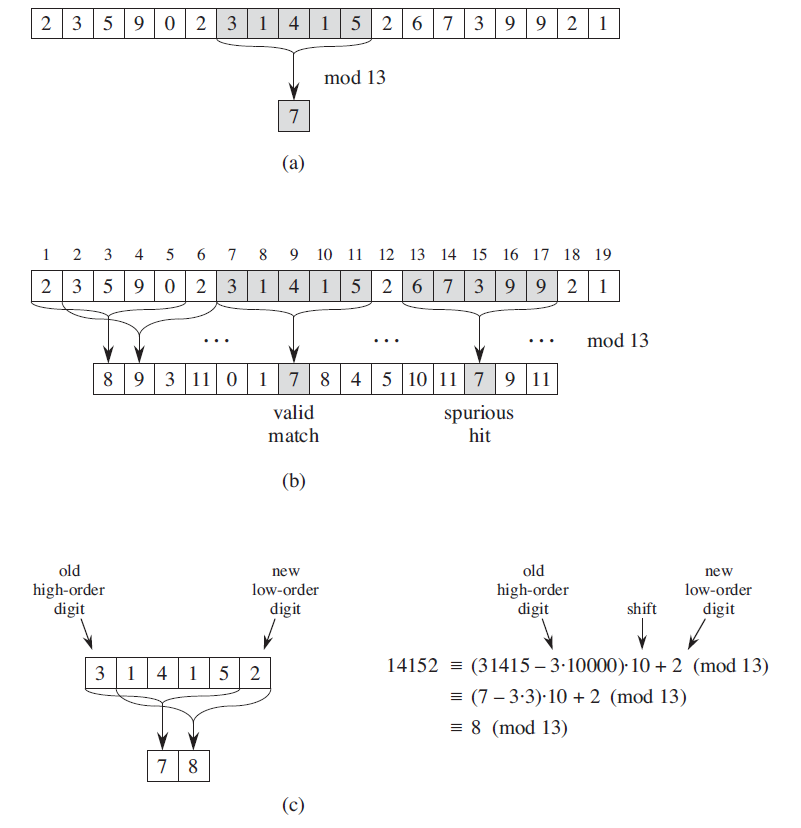
\includegraphics[scale=0.6]{./string_matching/pic1.PNG}
    \caption{$d = 10$, $q = 13$에 대한 라빈카프 알고리즘에 대한 수행을 나타낸다. (a)는 ``31415"에 대한 t가 7인모습 (b)는 숫자가 겹치지만 서로 다른 문자열에 대한것 (c)는 숫자비교를 끝낸후 다음 문자열에대한 변환을 나타낸 것이다.}
\end{figure}


수행시간을 개선하는 첫번째 아이디어는 문자를 숫자로 바꾸는것이다.
$111$과 $121$이란 문자열을 비교하려면 첫번째방법인 각 자리별로 3번 비교해야하지만 숫자로 비교하는건 한번만 비교하면된다.
따라서 문자열을 숫자로 바꾸기위한 전처리 시간이 든다.
전처리는 $P$패턴만을 $\Theta(m)$동안 바꾸고 문자열 $T$는 비교와 동시에 처리한다.

그다음 문자열을 어떻게 숫자로 나타낼까를 고민해야하는데 이때 문자가 나타내는 언어의 총갯수에대한 진법에서 10진법으로 변환한다. 따라서 실제 알고리즘을 실행할때 언어의 총갯수 $d$ $(|\Sigma|)$를 인자로 넣어주어야한다.
이때 숫자로 바꿀때 너무 긴 문자열을 숫자로 바꿀시에 나타나는 오버플로우를 감안해, 적당한 값으로 나눌 $q$를 채용한다.그래서 그 나타낸 숫자가 매칭이 이루어졌을때 실제로 같은 문자열인지 검사하는 부분이 필요하다. 이 $q$는 일반적으로 $dq$가 컴퓨터 한워드에 들어가는 소수로 채용한다.

호너의 법칙(Horner's law)을 사용해 다음의 수식으로 $\Theta(m)$시간에 패턴 $P$에대한 숫자 $p$를 전처리한다.

$$p = (dp+P[i]) \bmod q$$

문자열 $T[s+1..s+m]$에 대한 숫자 $t_s$의 처리는 매칭과 직후에 계산 한다.

$$t_{s+1} = (d(t_s - T[s+1]h) + T[s+m+1]) \bmod q$$

$ h = d^{m-1} \bmod q$이다. 가장 앞의 $T[s+1]$을 $h$를 곱해 제거하고 왼쪽으로 시프트 후 $T[s+m+1]$를 더하는 방식이다.



\begin{lstlisting}[style = CStyle]
RABIN-KARP-MATCHER(T,P,d,q)
    n = T.length
    m = P.length
    h = d^{m-1} mod q
    p = 0
    t_0 = 0
    for( i = 1 to m)
        p = (dp+P[i])mod q
        t_0 = (dt_0 + T[i]) mod q
    for s = 0 to n-m
        if p == t_s
            if P[1..m] == T[s+1..s+m]
                print ``Pattern occurs with shift s"
        if s < n - m
            t_{s+1} = (d(t_s - T[s+1]h) + T[s+m+1]) mod q
\end{lstlisting}

이 방법은 초기보다는 확실하게 개선되었지만 여전히 완벽하게 일치하는지 확인하기 위해 하나하나 비교하는 방법을 사용한다. 이상적인 경우는 $(m-n+a)$정도 돌겠지만  따라서 최악의 경우 매칭 시간이 $O((n-m+1)m)$이 된다.

\section{String matching with finite automata}

\begin{itemize}
    \item 전처리 $O(m|\Sigma|)$
    \item 매칭시간 $\Theta(n)$
\end{itemize}

\begin{dfn}[automata]
    finite automaton은 다음과 같이 5개의 튜플로 구성된다.
    \begin{itemize}
        \item $Q$ : 유한 상태의 집합
        \item $q_0$ :시작 상태 ($q_0 \in Q$)
        \item $A$ : 받아들이는 상태의 구분된 상태 ($A \subset Q$)
        \item $\Sigma$ : 유한 입력 알파벳
        \item $\delta$ : $Q \times \Sigma$에서 $Q$로 매핑되는 전이 함수 $M$    \end{itemize}
\end{dfn}

CLRS의 번역본을 그대로 들고왔습니다.


뭔소린지모르겠죠?

저도 그럼

오토마타 내용 통째로 생략

\newpage



\begin{figure}[h!]
    \centering
    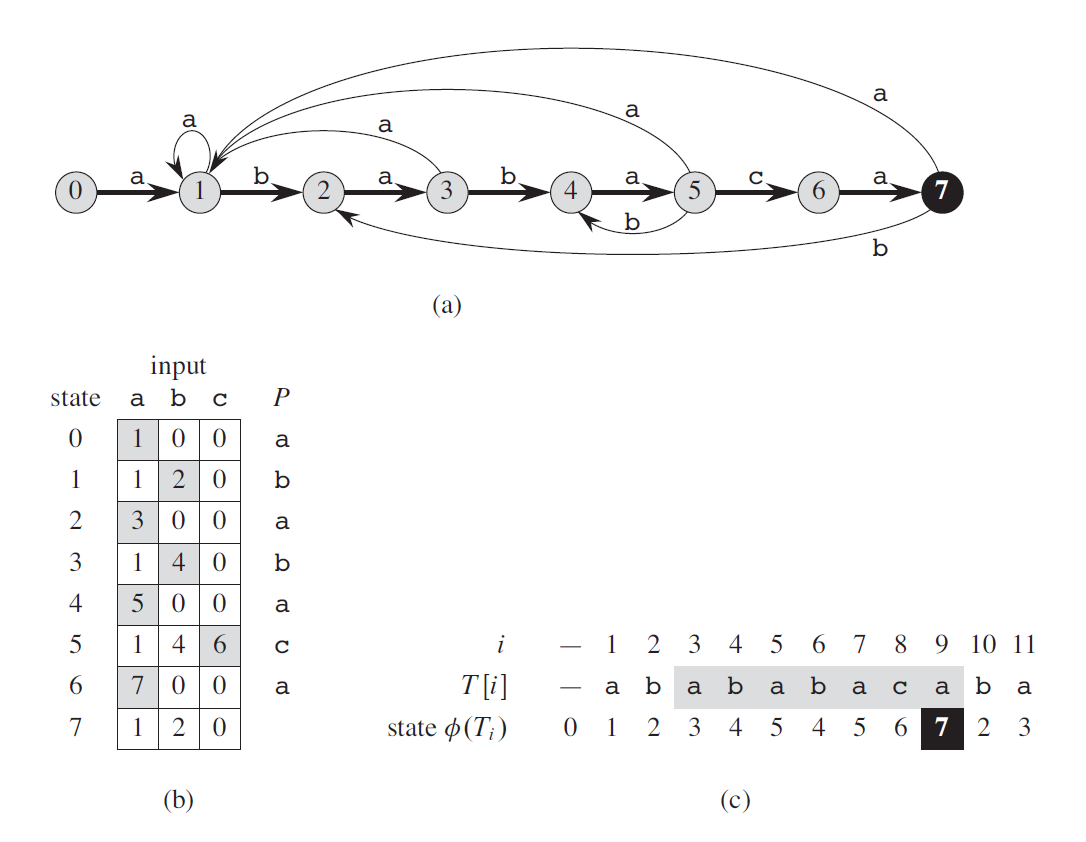
\includegraphics[scale=0.4]{./string_matching/pic2.PNG}
    \caption{$|\Sigma|  = 3$ ``a,b,c", $m = 7$에 대한 스트링 매칭 오토마타
    (a) 패턴 $P$에 대한 상태 오토마타 (b) 상태표 (c) 상태표에 따른 연산}
\end{figure}

오토마타를 이용한 스트링 매칭은 전처리에 일치한 앞 문자열 상태에 따른 상태표 $\delta$를 구하고 이를 이용해 매칭을 하는것이다.
상태는 $0,..,m$까지 있다. 초기 시작 상태는 0이고(매칭되는 알파벳이 하나도 없는 상태)
매칭되는 알파벳갯수에따라 상태 넘버를 가진다.

매칭시에 문자열 $T$는 각 자리마다 상태를 가진다. 각 상태를 가지고 다음에 나오는 문자에 따라 상태를 변화시키고 상태가 $m$에 도달하면 매칭이 된것으로 본다.

상태표의 특징은 상태가 변할때 일치한 문자열이 가장 길게 일치하는 상태로 보내는 것이다.
가령 그림 (c)에서 $T[5]$에서 $T[6]$으로 넘어갈때 ``ababa"까지 일치했지만 ``b"가 나옴으로써 매칭이 실패하지만 뒤에나온 ``b"를 포함해 ``abab"까지가 일치하기에 상태가 4로 돌아간것을 볼수있다.

\begin{lstlisting}[style = CStyle]
FINITE-AUTOMATON-MATCHER(T, delta , m)
n = T.length
q = 0 
for i = 1 to n
    q = d(q,T[i])
    if q == m
        print ``Pattern occurs with shift i-m"
\end{lstlisting}


상태표를 구하기위해서 다음과 같이 진행한다.
각 상태 $q$ 마다 각 알파벳 $a$를 뽑는다.
현재 상태 $q$의 문자열 + 'a'가 임의의 상태 $k$를 끝에서 포함하는지 검사하고 다를시 $k$를 계속 낮춰간다.

\begin{lstlisting}[style = CStyle]
COMPUTE-TRANSITION-FUNCTION(P, Sigma)
m = P.length
for q = 0 to m
    for a in Sigma
        k = min(m+1,q+2)
        repeat 
            k = k - 1
            until P_k ] P_q-a
            d(q,a) = k
return d
\end{lstlisting}



다음의 전처리의 수행시간은  $O(m^3 \Sigma)$이다.
뒷절의 $KMP$방식을 차용해서 $O(m \Sigma)$로 개선할수있다.


라빈 카프보다 확실히 개선된 방안을 가졌으며 전처리에 문자열 $T$의 개입또한 없다. 그러나 위의 전처리 시간은 $O(m^3 \Sigma)$이며, 상태표의 공간 복잡도의 크기가 $\Theta(m|\Sigma|)$만큼 필요하다.
다음 절에서 이를 더 줄여볼것이다.






\section{The Knuth-Morris-Pratt algorithm}

\begin{itemize}
    \item 전처리 : $O(m)$
    \item 매칭시간 : $\Theta(n)$
\end{itemize}


흔히 KMP 알고리즘이라 부르는데 이 알고리즘은 처음의 가장 기본적인 비교방식을 개선했다고 볼 수 있다. 전처리를 통해 계산한 $\pi[1..m]$ 배열을 사용하며, 매칭이 실패했을때, $\pi$배열을 사용한다.
\newpage
\begin{figure}[h!]
    \centering
    
\includegraphics[scale=0.7]{./string_matching/pic3.PNG}
    %\caption{}
\end{figure}

그림과 같이 ``ababaca"패턴을 문자열과 비교한다고 생각해보자.
``ababa"까지 맞지만 'c'와 문자가 일치하지 않는다. 이때 앞의 문자열은 ``ababa"가 패턴이 일치하는것은 자명하다. 이때 ``ababa"에 가장 근접하고 일치하는 수가 적은 $P$의 패턴이 ``aba"임을 알수있는 배열 $\pi[]$를 이용해서 다시 비교하지 않아도 ``aba"까지 일치함을 알수있다. 


\begin{figure}[h!]
    \centering
    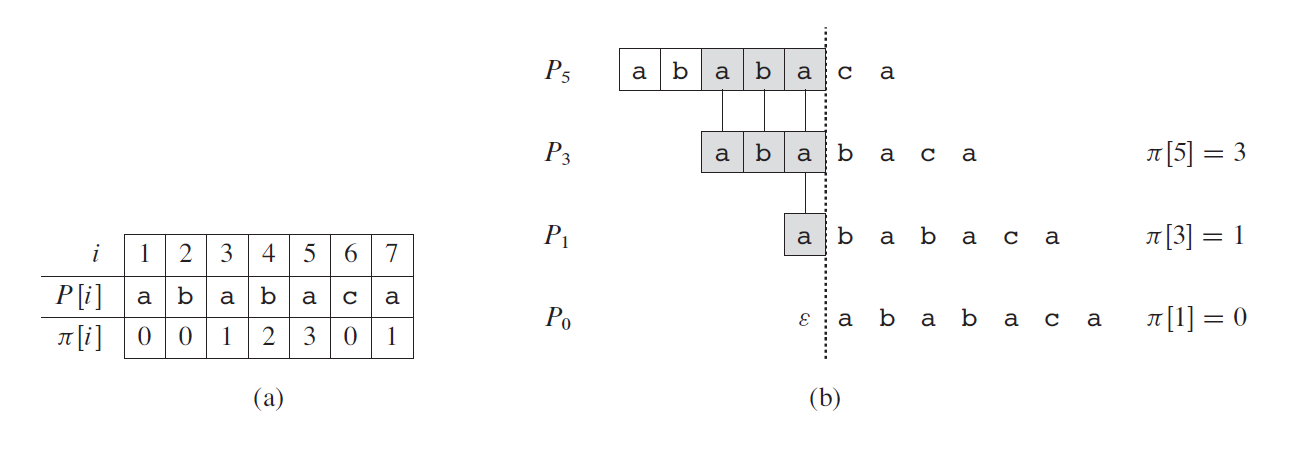
\includegraphics[scale=0.4]{./string_matching/pic4.PNG}
    \caption{(a)는 패턴 $P$와 전처리한 $\pi[1..7]$ (b)는 $P[5]$에서 다음 문자가 매칭이 틀렸을때 그에 따른 $\pi$값과 되돌아가는 순서를 나타낸것이다.}
\end{figure}


\begin{lstlisting}[style = CStyle]
KMP-MATCHER(T,P)
    n = T.length
    m = P:length
    PI[] = COMPUTE-PREFIX-FUNCTION(P)
    q = 0 // number of characters matched
    for i = 1 to n // scan the text from left to right
        while q>0 and P [q+1] != T[i]
            q = PI[q] // next character does not match  
        if P [q+1] == T[i]
            q = q + 1 // next character matches
        if q == m // is all of P matched?
            print ``Pattern occurs with shift" i - m
            q  = PI[q]
\end{lstlisting}



\begin{lstlisting}[style = CStyle]
COMPUTE-PREFIX-FUNCTION(P) /
m = P.length
let PI[1..m] be a new array
PI[1] = 0
k = 0
for q = 2 to m
    while k>0 and P[k+1] != P[q]
        k = P[k]
    if P[k+1] == P[q]
            k = k + 1
    PI[q] = k 
retunr PI
\end{lstlisting}

%----------------------------------------------------------------------------------------
%	INTRODUCTION SECTION
%----------------------------------------------------------------------------------------

\chapter*{Introduction/Prologue} % Introduction chapter suppressed from the table of contents

\begin{quote}
This is one of my finer quotations.\\
--John Smith
\end{quote}

This is a great place to write an introduction or prologue\footnote{You can even use a footnote to seem smarter}.

%----------------------------------------------------------------------------------------
%	BOOK PART
%----------------------------------------------------------------------------------------

\part{The Fairy Tales}

%----------------------------------------------------------------------------------------
%	CHAPTER ONE
%----------------------------------------------------------------------------------------

\chapter{Little Red Riding Hood}

Once upon a time there was a dear little girl who was loved by everyone who looked at her, but most of all by her grandmother, and there was nothing that she would not have given to the child. Once she gave her a little cap of red velvet, which suited her so well that she would never wear anything else; so she was always called `'

\begin{figure}[h!]
    \centering
    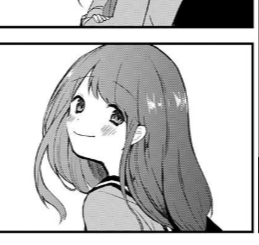
\includegraphics[scale=0.6]{pic5.PNG}
\end{figure}

One day her mother said to her: `Come, Little Red-Cap, here is a piece of cake and a bottle of wine; take them to your grandmother, she is ill and weak, and they will do her good. Set out before it gets hot, and when you are going, walk nicely and quietly and do not run off the path, or you may fall and break the bottle, and then your grandmother will get nothing; and when you go into her room, don't forget to say, ``Good morning'', and don't peep into every corner before you do it.'

`I will take great care,' said Little Red-Cap to her mother, and gave her hand on it.

% The grandmother lived out in the wood, half a league from the village, and just as Little Red-Cap entered the wood, a wolf met her. Red-Cap did not know what a wicked creature he was, and was not at all afraid of him.

% `Good day, Little Red-Cap,' said he.

% `Thank you kindly, wolf.'

% `Whither away so early, Little Red-Cap?'

% `To my grandmother's.'

% `What have you got in your apron?'

% `Cake and wine; yesterday was baking-day, so poor sick grandmother is to have something good, to make her stronger.'

% `Where does your grandmother live, Little Red-Cap?'

% `A good quarter of a league farther on in the wood; her house stands under the three large oak-trees, the nut-trees are just below; you surely must know it,' replied Little Red-Cap.

% The wolf thought to himself: `What a tender young creature! what a nice plump mouthful--she will be better to eat than the old woman. I must act craftily, so as to catch both.' So he walked for a short time by the side of Little Red-Cap, and then he said: `See, Little Red-Cap, how pretty the flowers are about here--why do you not look round? I believe, too, that you do not hear how sweetly the little birds are singing; you walk gravely along as if you were going to school, while everything else out here in the wood is merry.'

% Little Red-Cap raised her eyes, and when she saw the sunbeams dancing here and there through the trees, and pretty flowers growing everywhere, she thought: `Suppose I take grandmother a fresh nosegay; that would please her too. It is so early in the day that I shall still get there in good time'; and so she ran from the path into the wood to look for flowers. And whenever she had picked one, she fancied that she saw a still prettier one farther on, and ran after it, and so got deeper and deeper into the wood.

% Meanwhile the wolf ran straight to the grandmother's house and knocked at the door.

% `Who is there?'

% `Little Red-Cap,' replied the wolf. `She is bringing cake and wine; open the door.'

% `Lift the latch,' called out the grandmother, `I am too weak, and cannot get up.'

% The wolf lifted the latch, the door sprang open, and without saying a word he went straight to the grandmother's bed, and devoured her. Then he put on her clothes, dressed himself in her cap laid himself in bed and drew the curtains.

% Little Red-Cap, however, had been running about picking flowers, and when she had gathered so many that she could carry no more, she remembered her grandmother, and set out on the way to her.

% She was surprised to find the cottage-door standing open, and when she went into the room, she had such a strange feeling that she said to herself: `Oh dear! how uneasy I feel today, and at other times I like being with grandmother so much.' She called out: `Good morning,' but received no answer; so she went to the bed and drew back the curtains. There lay her grandmother with her cap pulled far over her face, and looking very strange.

% `Oh! grandmother,' she said, `what big ears you have!'

% `The better to hear you with, my child,' was the reply.

% `But, grandmother, what big eyes you have!' she said.

% `The better to see you with, my dear.'

% `But, grandmother, what large hands you have!'

% `The better to hug you with.'

% `Oh! but, grandmother, what a terrible big mouth you have!'

% `The better to eat you with!'

% And scarcely had the wolf said this, than with one bound he was out of bed and swallowed up Red-Cap.

% When the wolf had appeased his appetite, he lay down again in the bed, fell asleep and began to snore very loud. The huntsman was just passing the house, and thought to himself: `How the old woman is snoring! I must just see if she wants anything.' So he went into the room, and when he
% came to the bed, he saw that the wolf was lying in it. `Do I find you here, you old sinner!' said he. `I have long sought you!' Then just as he was going to fire at him, it occurred to him that the wolf might have devoured the grandmother, and that she might still be saved, so he did not fire, but took a pair of scissors, and began to cut open the stomach of the sleeping wolf. When he had made two snips, he saw the little Red-Cap shining, and then he made two snips more, and the little girl sprang out, crying: `Ah, how frightened I have been! How dark it was inside the wolf'; and after that the aged grandmother came out alive also, but scarcely able to breathe. Red-Cap, however, quickly fetched
% great stones with which they filled the wolf's belly, and when he awoke, he wanted to run away, but the stones were so heavy that he collapsed at once, and fell dead.

% Then all three were delighted. The huntsman drew off the wolf's skin and went home with it; the grandmother ate the cake and drank the wine which Red-Cap had brought, and revived, but Red-Cap thought to herself: `As long as I live, I will never by myself leave the path, to run into the wood, when my mother has forbidden me to do so.'

% It also related that once when Red-Cap was again taking cakes to the old grandmother, another wolf spoke to her, and tried to entice her from the path. Red-Cap, however, was on her guard, and went straight forward on her way, and told her grandmother that she had met the wolf, and that he had said `good morning' to her, but with such a wicked look in his eyes, that if they had not been on the public road she was certain he would have eaten her up. `Well,' said the grandmother, `we will shut the door, that he may not come in.' Soon afterwards the wolf knocked, and cried: `Open the door, grandmother, I am Little Red-Cap, and am bringing you some cakes.' But they did not speak, or open the door, so the grey-beard stole twice or thrice round the house, and at last jumped on the roof, intending to wait until Red-Cap went home in the evening, and then to steal after her and devour her in the darkness. But the grandmother saw what was in his thoughts. In front of the house was a great stone trough, so she said to the child: `Take the pail, Red-Cap; I made some sausages yesterday, so carry the water in which I boiled them to the trough.' Red-Cap carried until the great trough was quite full. Then the smell of the sausages reached the wolf, and he sniffed and peeped down, and at last stretched out his neck so far that he could no longer keep his footing and began to slip, and slipped down from the roof straight into the great trough, and was drowned. But Red-Cap went joyously home, and no one ever did anything to harm her again.

% %----------------------------------------------------------------------------------------
% %	CHAPTER TWO
% %----------------------------------------------------------------------------------------

% \chapter{Hansel and Gretel}

% Hard by a great forest dwelt a poor wood-cutter with his wife and his two children. The boy was called Hansel and the girl Gretel. He had little to bite and to break, and once when great dearth fell on the land, he could no longer procure even daily bread. Now when he thought over this by night in his bed, and tossed about in his anxiety, he groaned and said to his wife: `What is to become of us? How are we to feed our poor children, when we no longer have anything even for ourselves?' `I'll tell you what, husband,' answered the woman, `early tomorrow morning we will take the children out into the forest to where it is the thickest; there we will light a fire for them, and give each of them one more piece of bread, and then we will go to our work and leave them alone. They will not find the way home again, and we shall be rid of them.' `No, wife,' said the man, `I will not do that; how can I bear to leave my children alone in the forest?--the wild animals would soon come and tear them to pieces.' `O, you fool!' said she, `then we must all four die of hunger, you may as well plane the planks for our coffins,' and she left him no peace until he consented. `But I feel very sorry for the poor children, all the same,' said the man.

% The two children had also not been able to sleep for hunger, and had heard what their stepmother had said to their father. Gretel wept bitter tears, and said to Hansel: `Now all is over with us.' `Be quiet, Gretel,' said Hansel, `do not distress yourself, I will soon find a way to help us.' And when the old folks had fallen asleep, he got up, put on his little coat, opened the door below, and crept outside. The moon shone brightly, and the white pebbles which lay in front of the house glittered like real silver pennies. Hansel stooped and stuffed the little pocket of his coat with as many as he could get in. Then he went back and said to Gretel: `Be comforted, dear little sister, and sleep in peace, God will not forsake us,' and he lay down again in his bed. When day dawned, but before the sun had risen, the woman came and awoke the two children, saying: `Get up, you sluggards! we are going into the forest to fetch wood.' She gave each a little piece of bread, and said: `There is something for your dinner, but do not eat it up before then, for you will get nothing else.' Gretel took the bread under her apron, as Hansel had the pebbles in his pocket. Then they all set out together on the way to the forest. When they had walked a short time, Hansel stood still and peeped back at the house, and did so again and again. His father said: `Hansel, what are you looking at there and staying behind for? Pay attention, and do not forget how to use your legs.' `Ah, father,' said Hansel, `I am looking at my little white cat, which is sitting up on the roof, and wants to say goodbye to me.' The wife said: Fool, that is not your little cat, that is the morning sun which is shining on the chimneys.' Hansel, however, had not been looking back at the cat, but had been constantly throwing one of the white pebble-stones out of his pocket on the road.

% When they had reached the middle of the forest, the father said: `Now, children, pile up some wood, and I will light a fire that you may not be cold.' Hansel and Gretel gathered brushwood together, as high as a little hill. The brushwood was lighted, and when the flames were burning very high, the woman said: `Now, children, lay yourselves down by the fire and rest, we will go into the forest and cut some wood. When we have done, we will come back and fetch you away.'

% Hansel and Gretel sat by the fire, and when noon came, each ate a little piece of bread, and as they heard the strokes of the wood-axe they believed that their father was near. It was not the axe, however, but a branch which he had fastened to a withered tree which the wind was blowing backwards and forwards. And as they had been sitting such a long time, their eyes closed with fatigue, and they fell fast asleep. When at last they awoke, it was already dark night. Gretel began to cry and said: `How are we to get out of the forest now?' But Hansel comforted her and said: `Just wait a little, until the moon has risen, and then we will soon find the way.' And when the full moon had risen, Hansel took his little sister by the hand, and followed the pebbles which shone like newly-coined silver pieces, and showed them the way.

% They walked the whole night long, and by break of day came once more to their father's house. They knocked at the door, and when the woman opened it and saw that it was Hansel and Gretel, she said: `You naughty children, why have you slept so long in the forest?--we thought you were never coming back at all!' The father, however, rejoiced, for it had cut him to the heart to leave them behind alone.

% Not long afterwards, there was once more great dearth throughout the land, and the children heard their mother saying at night to their father: `Everything is eaten again, we have one half loaf left, and that is the end. The children must go, we will take them farther into the wood, so that they will not find their way out again; there is no other means of saving ourselves!' The man's heart was heavy, and he thought: `It would be better for you to share the last mouthful with your children.' The woman, however, would listen to nothing that he had to say, but scolded and reproached him. He who says A must say B, likewise, and as he had yielded the first time, he had to do so a second time also.

% The children, however, were still awake and had heard the conversation. When the old folks were asleep, Hansel again got up, and wanted to go out and pick up pebbles as he had done before, but the woman had locked the door, and Hansel could not get out. Nevertheless he comforted his little sister, and said: `Do not cry, Gretel, go to sleep quietly, the good God will help us.'

% Early in the morning came the woman, and took the children out of their beds. Their piece of bread was given to them, but it was still smaller than the time before. On the way into the forest Hansel crumbled his in his pocket, and often stood still and threw a morsel on the ground. `Hansel, why do you stop and look round?' said the father, `go on.' `I am looking back at my little pigeon which is sitting on the roof, and wants to say goodbye to me,' answered Hansel. `Fool!' said the woman, `that is not your little pigeon, that is the morning sun that is shining on the chimney.' Hansel, however little by little, threw all the crumbs on the path.

% The woman led the children still deeper into the forest, where they had never in their lives been before. Then a great fire was again made, and the mother said: `Just sit there, you children, and when you are tired you may sleep a little; we are going into the forest to cut wood, and in the evening when we are done, we will come and fetch you away.' When it was noon, Gretel shared her piece of bread with Hansel, who had scattered his by the way. Then they fell asleep and evening passed, but no one came to the poor children. They did not awake until it was dark night, and Hansel comforted his little sister and said: `Just wait, Gretel, until the moon rises, and then we shall see the crumbs of bread which I have strewn about, they will show us our way home again.' When the moon came they set out, but they found no crumbs, for the many thousands of birds which fly about in the woods and fields had picked them all up. Hansel said to Gretel: `We shall soon find the way,' but they did not find it. They walked the whole night and all the next day too from morning till evening, but they did not get out of the forest, and were very hungry, for they had nothing to eat but two or three berries, which grew on the ground. And as they were so weary that their legs would carry them no longer, they lay down beneath a tree and fell asleep.

% It was now three mornings since they had left their father's house. They began to walk again, but they always came deeper into the forest, and if help did not come soon, they must die of hunger and weariness. When it was mid-day, they saw a beautiful snow-white bird sitting on a bough, which sang so delightfully that they stood still and listened to it. And when its song was over, it spread its wings and flew away before them, and they followed it until they reached a little house, on the roof of
% which it alighted; and when they approached the little house they saw that it was built of bread and covered with cakes, but that the windows were of clear sugar. `We will set to work on that,' said Hansel, `and have a good meal. I will eat a bit of the roof, and you Gretel, can eat some of the window, it will taste sweet.' Hansel reached up above, and broke off a little of the roof to try how it tasted, and Gretel leant against the window and nibbled at the panes. Then a soft voice cried
% from the parlour:

% 'Nibble, nibble, gnaw,
% Who is nibbling at my little house?'

% The children answered:

% 'The wind, the wind,
% The heaven-born wind,'

% and went on eating without disturbing themselves. Hansel, who liked the taste of the roof, tore down a great piece of it, and Gretel pushed out the whole of one round window-pane, sat down, and enjoyed herself with it. Suddenly the door opened, and a woman as old as the hills, who supported herself on crutches, came creeping out. Hansel and Gretel were so terribly frightened that they let fall what they had in their hands. The old woman, however, nodded her head, and said: `Oh, you dear children, who has brought you here? do come in, and stay with me. No harm shall happen to you.' She took them both by the hand, and led them into her little house. Then good food was set before them, milk and pancakes, with sugar, apples, and nuts. Afterwards two pretty little beds were covered with clean white linen, and Hansel and Gretel lay down in them, and thought they were in heaven.

% The old woman had only pretended to be so kind; she was in reality a wicked witch, who lay in wait for children, and had only built the little house of bread in order to entice them there. When a child fell into her power, she killed it, cooked and ate it, and that was a feast day with her. Witches have red eyes, and cannot see far, but they have a keen scent like the beasts, and are aware when human beings draw near. When Hansel and Gretel came into her neighbourhood, she laughed with
% malice, and said mockingly: `I have them, they shall not escape me again!' Early in the morning before the children were awake, she was already up, and when she saw both of them sleeping and looking so pretty, with their plump and rosy cheeks she muttered to herself: `That will be a dainty mouthful!' Then she seized Hansel with her shrivelled hand, carried him into a little stable, and locked him in behind a grated door. Scream as he might, it would not help him. Then she went to
% Gretel, shook her till she awoke, and cried: `Get up, lazy thing, fetch some water, and cook something good for your brother, he is in the stable outside, and is to be made fat. When he is fat, I will eat him.' Gretel began to weep bitterly, but it was all in vain, for she was forced to do what the wicked witch commanded.

% And now the best food was cooked for poor Hansel, but Gretel got nothing but crab-shells. Every morning the woman crept to the little stable, and cried: `Hansel, stretch out your finger that I may feel if you will soon be fat.' Hansel, however, stretched out a little bone to her, and the old woman, who had dim eyes, could not see it, and thought it was Hansel's finger, and was astonished that there was no way of fattening him. When four weeks had gone by, and Hansel still remained thin, she
% was seized with impatience and would not wait any longer. `Now, then, Gretel,' she cried to the girl, `stir yourself, and bring some water. Let Hansel be fat or lean, tomorrow I will kill him, and cook him.' Ah, how the poor little sister did lament when she had to fetch the water, and how her tears did flow down her cheeks! `Dear God, do help us,' she cried. `If the wild beasts in the forest had but devoured us, we should at any rate have died together.' `Just keep your noise to yourself,' said the old woman, `it won't help you at all.'

% Early in the morning, Gretel had to go out and hang up the cauldron with the water, and light the fire. `We will bake first,' said the old woman, `I have already heated the oven, and kneaded the dough.' She pushed poor Gretel out to the oven, from which flames of fire were already darting. `Creep in,' said the witch, `and see if it is properly heated, so that we can put the bread in.' And once Gretel was inside, she intended to shut the oven and let her bake in it, and then she would eat her, too. But Gretel saw what she had in mind, and said: `I do not know how I am to do it; how do I get in?' `Silly goose,' said the old woman. `The door is big enough; just look, I can get in myself!' and she crept up and thrust her head into the oven. Then Gretel gave her a push that drove her far into it, and shut the iron door, and fastened the bolt. Oh! then she began to howl quite horribly, but Gretel ran away and the godless witch was miserably burnt to death.

% Gretel, however, ran like lightning to Hansel, opened his little stable, and cried: `Hansel, we are saved! The old witch is dead!' Then Hansel sprang like a bird from its cage when the door is opened. How they did rejoice and embrace each other, and dance about and kiss each other! And as they had no longer any need to fear her, they went into the witch's house, and in every corner there stood chests full of pearls and jewels. `These are far better than pebbles!' said Hansel, and thrust into his
% pockets whatever could be got in, and Gretel said: `I, too, will take something home with me,' and filled her pinafore full. `But now we must be off,' said Hansel, `that we may get out of the witch's forest.'

% When they had walked for two hours, they came to a great stretch of water. `We cannot cross,' said Hansel, `I see no foot-plank, and no bridge.' `And there is also no ferry,' answered Gretel, 'but a white
% duck is swimming there: if I ask her, she will help us over.' Then she cried:

% 'Little duck, little duck, dost thou see,
% Hansel and Gretel are waiting for thee?
% There's never a plank, or bridge in sight,
% Take us across on thy back so white.'

% The duck came to them, and Hansel seated himself on its back, and told his sister to sit by him. `No,' replied Gretel, `that will be too heavy for the little duck; she shall take us across, one after the other.' The good little duck did so, and when they were once safely across and had walked for a short time, the forest seemed to be more and more familiar to them, and at length they saw from afar their father's house. Then they began to run, rushed into the parlour, and threw themselves round their father's neck. The man had not known one happy hour since he had left the children in the forest; the woman, however, was dead. Gretel emptied her pinafore until pearls and precious stones ran about the room, and Hansel threw one handful after another out of his pocket to add to them. Then all anxiety was at an end, and they lived together in perfect happiness. My tale is done, there runs a mouse; whosoever catches it, may make himself a big fur cap out of it.

% %----------------------------------------------------------------------------------------
% %	CHAPTER THREE
% %----------------------------------------------------------------------------------------

% \chapter{Rupunzel}

% There were once a man and a woman who had long in vain wished for a child. At length the woman hoped that God was about to grant her desire. These people had a little window at the back of their house from which a splendid garden could be seen, which was full of the most beautiful flowers and herbs. It was, however, surrounded by a high wall, and no one dared to go into it because it belonged to an enchantress, who had great power and was dreaded by all the world. One day the woman was standing by this window and looking down into the garden, when she saw a bed which was planted with the most beautiful rampion (rapunzel), and it looked so fresh and green that she longed for it, she quite pined away, and began to look pale and miserable. Then her husband was alarmed, and asked: `What ails you, dear wife?' `Ah,' she replied, `if I can't eat some of the rampion, which is in the garden behind our house, I shall die.' The man, who loved her, thought: `Sooner than let your wife die, bring her some of the rampion yourself, let it cost what it will.' At twilight, he clambered down over the wall into the garden of the enchantress, hastily clutched a handful of rampion, and took it to his wife. She at once made herself a salad of it, and ate it greedily. It tasted so good to her--so very good, that the next day she longed for it three times as much as before. If he was to have any rest, her husband must once more descend into the garden. In the gloom of evening therefore, he let himself down again; but when he had clambered down the wall he was terribly afraid, for he saw the enchantress standing before him. `How can you dare,' said she with angry look, `descend into my garden and steal my rampion like a thief? You shall suffer for it!' `Ah,' answered he, `let mercy take the place of justice, I only made up my mind to do it out of necessity. My wife saw your rampion from the window, and felt such a longing for it that she would have died if she had not got some to eat.' Then the enchantress allowed her anger to be softened, and said to him: `If the case be as you say, I will allow you to take away with you as much rampion as you will, only I make one condition, you must give me the child which your wife will bring into the world; it shall be well treated, and I will care for it like a mother.' The man in his terror consented to everything, and when the woman was brought to bed, the enchantress appeared at once, gave the child the name of Rapunzel, and took it away with her.

% Rapunzel grew into the most beautiful child under the sun. When she was twelve years old, the enchantress shut her into a tower, which lay in a forest, and had neither stairs nor door, but quite at the top was a little window. When the enchantress wanted to go in, she placed herself beneath it and cried:

% 'Rapunzel, Rapunzel,
% Let down your hair to me.'

% Rapunzel had magnificent long hair, fine as spun gold, and when she heard the voice of the enchantress she unfastened her braided tresses, wound them round one of the hooks of the window above, and then the hair fell twenty ells down, and the enchantress climbed up by it.

% After a year or two, it came to pass that the king's son rode through the forest and passed by the tower. Then he heard a song, which was so charming that he stood still and listened. This was Rapunzel, who in her solitude passed her time in letting her sweet voice resound. The king's son wanted to climb up to her, and looked for the door of the tower, but none was to be found. He rode home, but the singing had so deeply touched his heart, that every day he went out into the forest and listened to it. Once when he was thus standing behind a tree, he saw that an enchantress came there, and he heard how she cried:

% 'Rapunzel, Rapunzel,
% Let down your hair to me.'

% Then Rapunzel let down the braids of her hair, and the enchantress climbed up to her. `If that is the ladder by which one mounts, I too will try my fortune,' said he, and the next day when it began to grow dark, he went to the tower and cried:

% 'Rapunzel, Rapunzel,
% Let down your hair to me.'

% Immediately the hair fell down and the king's son climbed up.

% At first Rapunzel was terribly frightened when a man, such as her eyes had never yet beheld, came to her; but the king's son began to talk to her quite like a friend, and told her that his heart had been so stirred that it had let him have no rest, and he had been forced to see her. Then Rapunzel lost her fear, and when he asked her if she would take him for her husband, and she saw that he was young and handsome, she thought: `He will love me more than old Dame Gothel does'; and she said
% yes, and laid her hand in his. She said: `I will willingly go away with you, but I do not know how to get down. Bring with you a skein of silk every time that you come, and I will weave a ladder with it, and when that is ready I will descend, and you will take me on your horse.' They agreed that until that time he should come to her every evening, for the old woman came by day. The enchantress remarked nothing of this, until once Rapunzel said to her: `Tell me, Dame Gothel, how it happens that you are so much heavier for me to draw up than the young king's son--he is with me in a moment.' `Ah! you wicked child,' cried the enchantress. `What do I hear you say! I thought I had separated you from all the world, and yet you have deceived me!' In her anger she clutched Rapunzel's beautiful tresses, wrapped them twice round her left hand, seized a pair of scissors with the right, and snip, snap, they were cut off, and the lovely braids lay on the ground. And she was so pitiless that she took poor Rapunzel into a desert where she had to live in great grief and misery.

% On the same day that she cast out Rapunzel, however, the enchantress fastened the braids of hair, which she had cut off, to the hook of the window, and when the king's son came and cried:

% 'Rapunzel, Rapunzel,
% Let down your hair to me.'

% she let the hair down. The king's son ascended, but instead of finding his dearest Rapunzel, he found the enchantress, who gazed at him with wicked and venomous looks. `Aha!' she cried mockingly, 'you would fetch your dearest, but the beautiful bird sits no longer singing in the nest;
% the cat has got it, and will scratch out your eyes as well. Rapunzel is lost to you; you will never see her again.' The king's son was beside himself with pain, and in his despair he leapt down from the tower. He escaped with his life, but the thorns into which he fell pierced his eyes. Then he wandered quite blind about the forest, ate nothing but roots and berries, and did naught but lament and weep over the loss of his dearest wife. Thus he roamed about in misery for some years, and at
% length came to the desert where Rapunzel, with the twins to which she had given birth, a boy and a girl, lived in wretchedness. He heard a voice, and it seemed so familiar to him that he went towards it, and when he approached, Rapunzel knew him and fell on his neck and wept. Two of her tears wetted his eyes and they grew clear again, and he could see with them as before. He led her to his kingdom where he was joyfully received, and they lived for a long time afterwards, happy and contented.

% %----------------------------------------------------------------------------------------

\end{document}